\chapter{Requisitos do Sistema}

\section{Análise e Levantamento dos Requisitos}
\subsection{Criação do grupo com os elementos da casa/apartamento}
A aplicação a desenvolver deverá suportar o registo das despesas e a gestão do seu pagamento por parte de moradores registados. Para tal é necessário que cada morador efetue um regiso fornecendo o seu nome, e-mail, número de telemóvel e data de nascimento. Após o registo será associada uma conta corrente, esta que permitirá a gestão do saldo (estão incluidas dividas) de cada morador. 


\subsection{Gestão das contas}
 O morador deverá efetuar um pagamento, que será creditado na conta corrente do morador. 
 
 O pagamento pode ser efetuado com valores relativamente grandes ao qual é debitado consoante é necessário ou depósitos da quantia necessária para pagar a/s despesa/s em causa. 
 
 Existirá um saldo global da casa, este que é o somatório de todas as contas correntes dos moradores, este saldo é administrado por um Adminstrador. 
 
 Existem dois tipos de despesas distintos: a despesa recorrente referente a despesas mensais como a água, luz, renda, etc; 
 a despesa extra referente a por exemplo arranjos de material na casa. 
 
 Cada morador deverá pagar uma fração relativa à despesa. 
 
 Cada despesa a pagar tem a si associado um tipo. 
 
 

\section{Base de dados }
A aplicação necessitará de uma implementação de uma base de dados para gerir os elementos que pertencem ao grupo assim como as despesas efetuadas pelos moradores. 

\chapter{Arquitetura da Aplicação}


\section{Modelo de Dominio }
Todo e qualquer projeto possui um domínio específico. O modelo de domínio deve capturar os seguintes pontos: as entidades, os relacionamentos entre as entidades e o vocabulário de domínio do problema. Para além disso também deve ser uma visão estática do problema onde é possível representar as regras de negócio invariantes no tempo. Ou seja, o modelo de domínio é a base para a análise de requisitos.

No que diz respeito à aplicação, como é dito na introdução, queremos desenvolver uma aplicação capaz de suportar o registo das despesas e a gestão do seu pagamento por parte dos moradores registados.


\begin{figure}[htb!]
	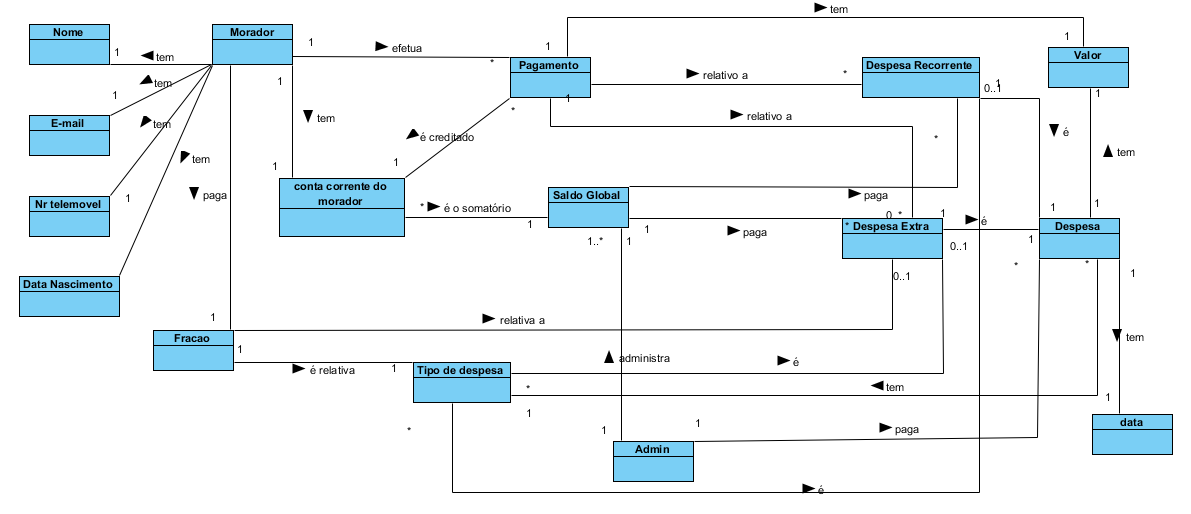
\includegraphics[scale=0.566]{modelodominio}  
	\caption{Modelo Dominio}  
\end{figure}


\section{Diagramas de Use Case}


\begin{figure}[htb!]
	\centering
	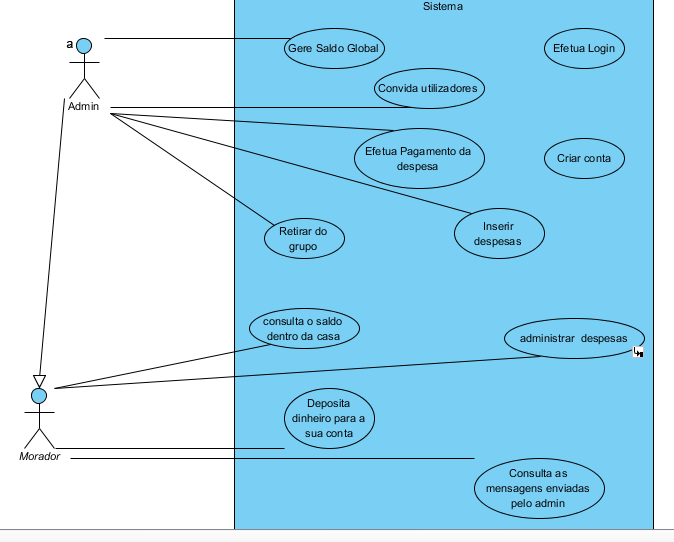
\includegraphics[scale=0.7]{usecase1}  
	\caption{Modelo Use Case}  
\end{figure}


\newpage
\section{Mockups}




